%!TEX root = ../DissertationDefensePresentation.tex

%%--------------------------------------------------------------------------------------------

\subsection*{LHC}

%%--------------------------------------------------------------------------------------------

\frame{
    \frametitle{The Large Hadron Collider (LHC)}
    \vspace*{-0.24cm}
    \begin{columns}[T]
        \column{0.58\textwidth}
            \vspace*{-0.25cm}
            \begin{block}{}
                \begin{itemize}
                    \footnotesize
                    \item Proton-proton collider near Geneva, Switzerland
                    \begin{itemize}
                        \scriptsize
                        \item Design center of mass energy of 14\TeV
                        \item 27\unit{km} circumference and $\sim$100\unit{m} under the French-Swiss border
                    \end{itemize}
                    \item This analysis uses the full 2012 dataset
                    \begin{itemize}
                        \scriptsize
                        \item \CM{8\tev}
                        \item $\int \mathcal{L}\sim$19.148 (19.279)\fbinv for electrons (muons)
                    \end{itemize}
                    \item Two general purpose detectors (\textbf{CMS} \& ATLAS) and several other specialized experiments
                \end{itemize}
            \end{block}
            \begin{center}
                \vspace*{-0.25cm}
                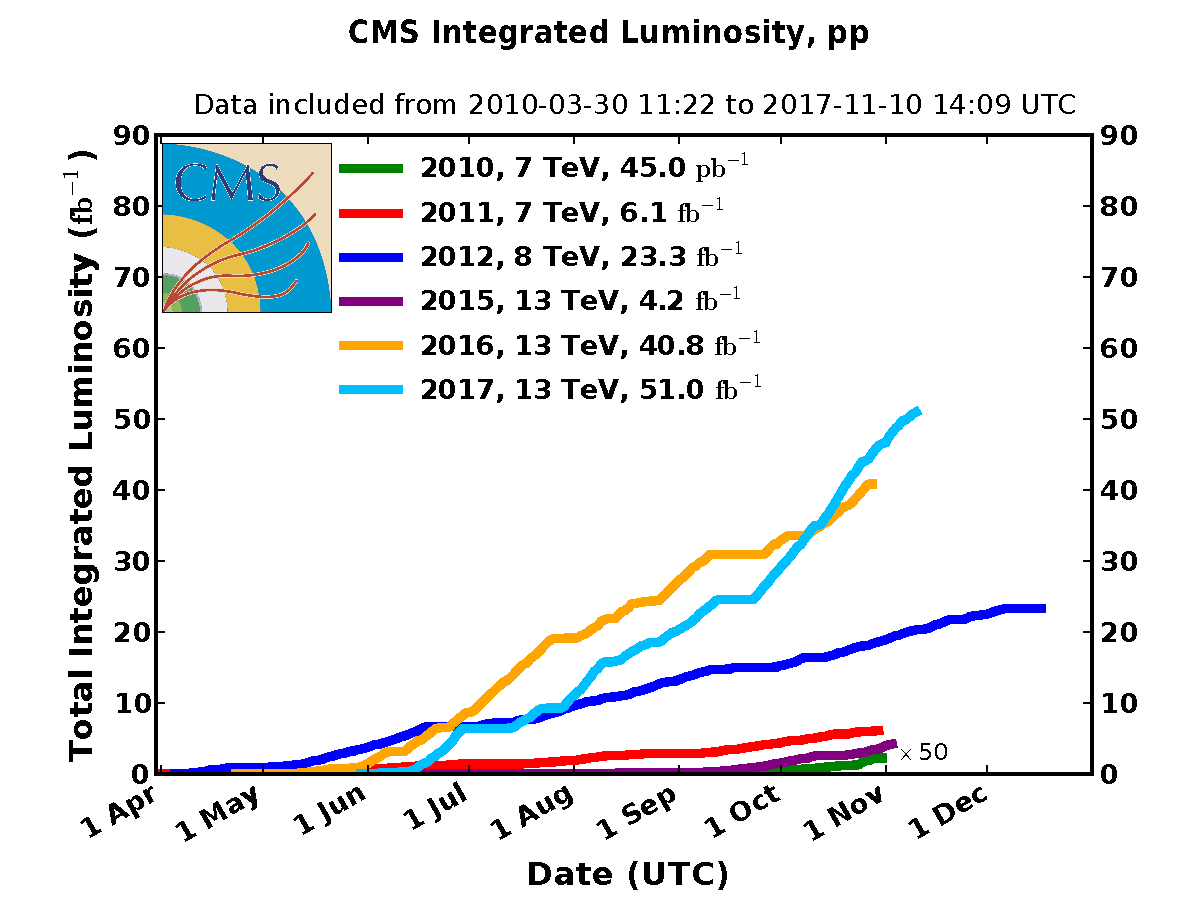
\includegraphics[width=0.83\textwidth]{\figpath/int_lumi_cumulative_pp_2.pdf}
            \end{center}
        \column{0.4\textwidth}
            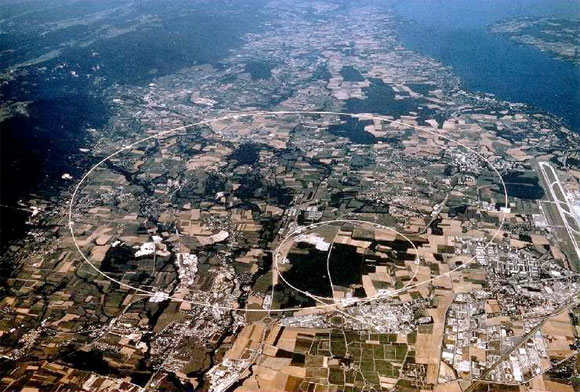
\includegraphics[width=\figwidth]{\figpath/cern_lhc.jpg}\\
            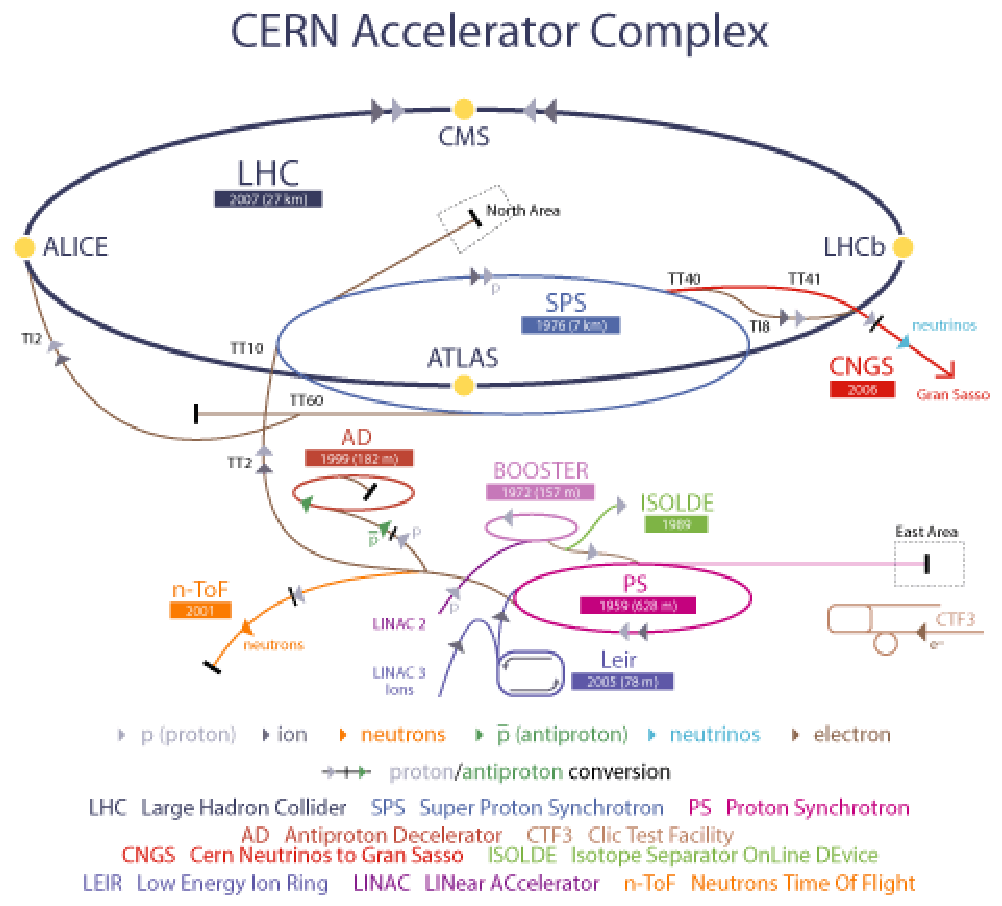
\includegraphics[width=\figwidth]{\figpath/AccComplex.pdf}
    \end{columns}
}

%%--------------------------------------------------------------------------------------------

\subsection*{Compact Muon Solenoid (CMS)}

%%--------------------------------------------------------------------------------------------

\frame{
    \frametitle{The Compact Muon Solenoid (CMS)}
    \vspace*{-0.24cm}
    \begin{block}{}
        \begin{itemize}
            \small
            \item Standard multipurpose detector, benefits from:
            \begin{itemize}
                \footnotesize
                \item High magnetic field
                \item High granularity tracker (lepton finding)
                \item Excellent electromagnetic calorimeter resolution
                \item Good particle identification due to the particle flow (PF) algorithm
            \end{itemize}            
        \end{itemize}
    \end{block}
    \begin{columns}[T]
        \begin{column}{0.65\textwidth}
            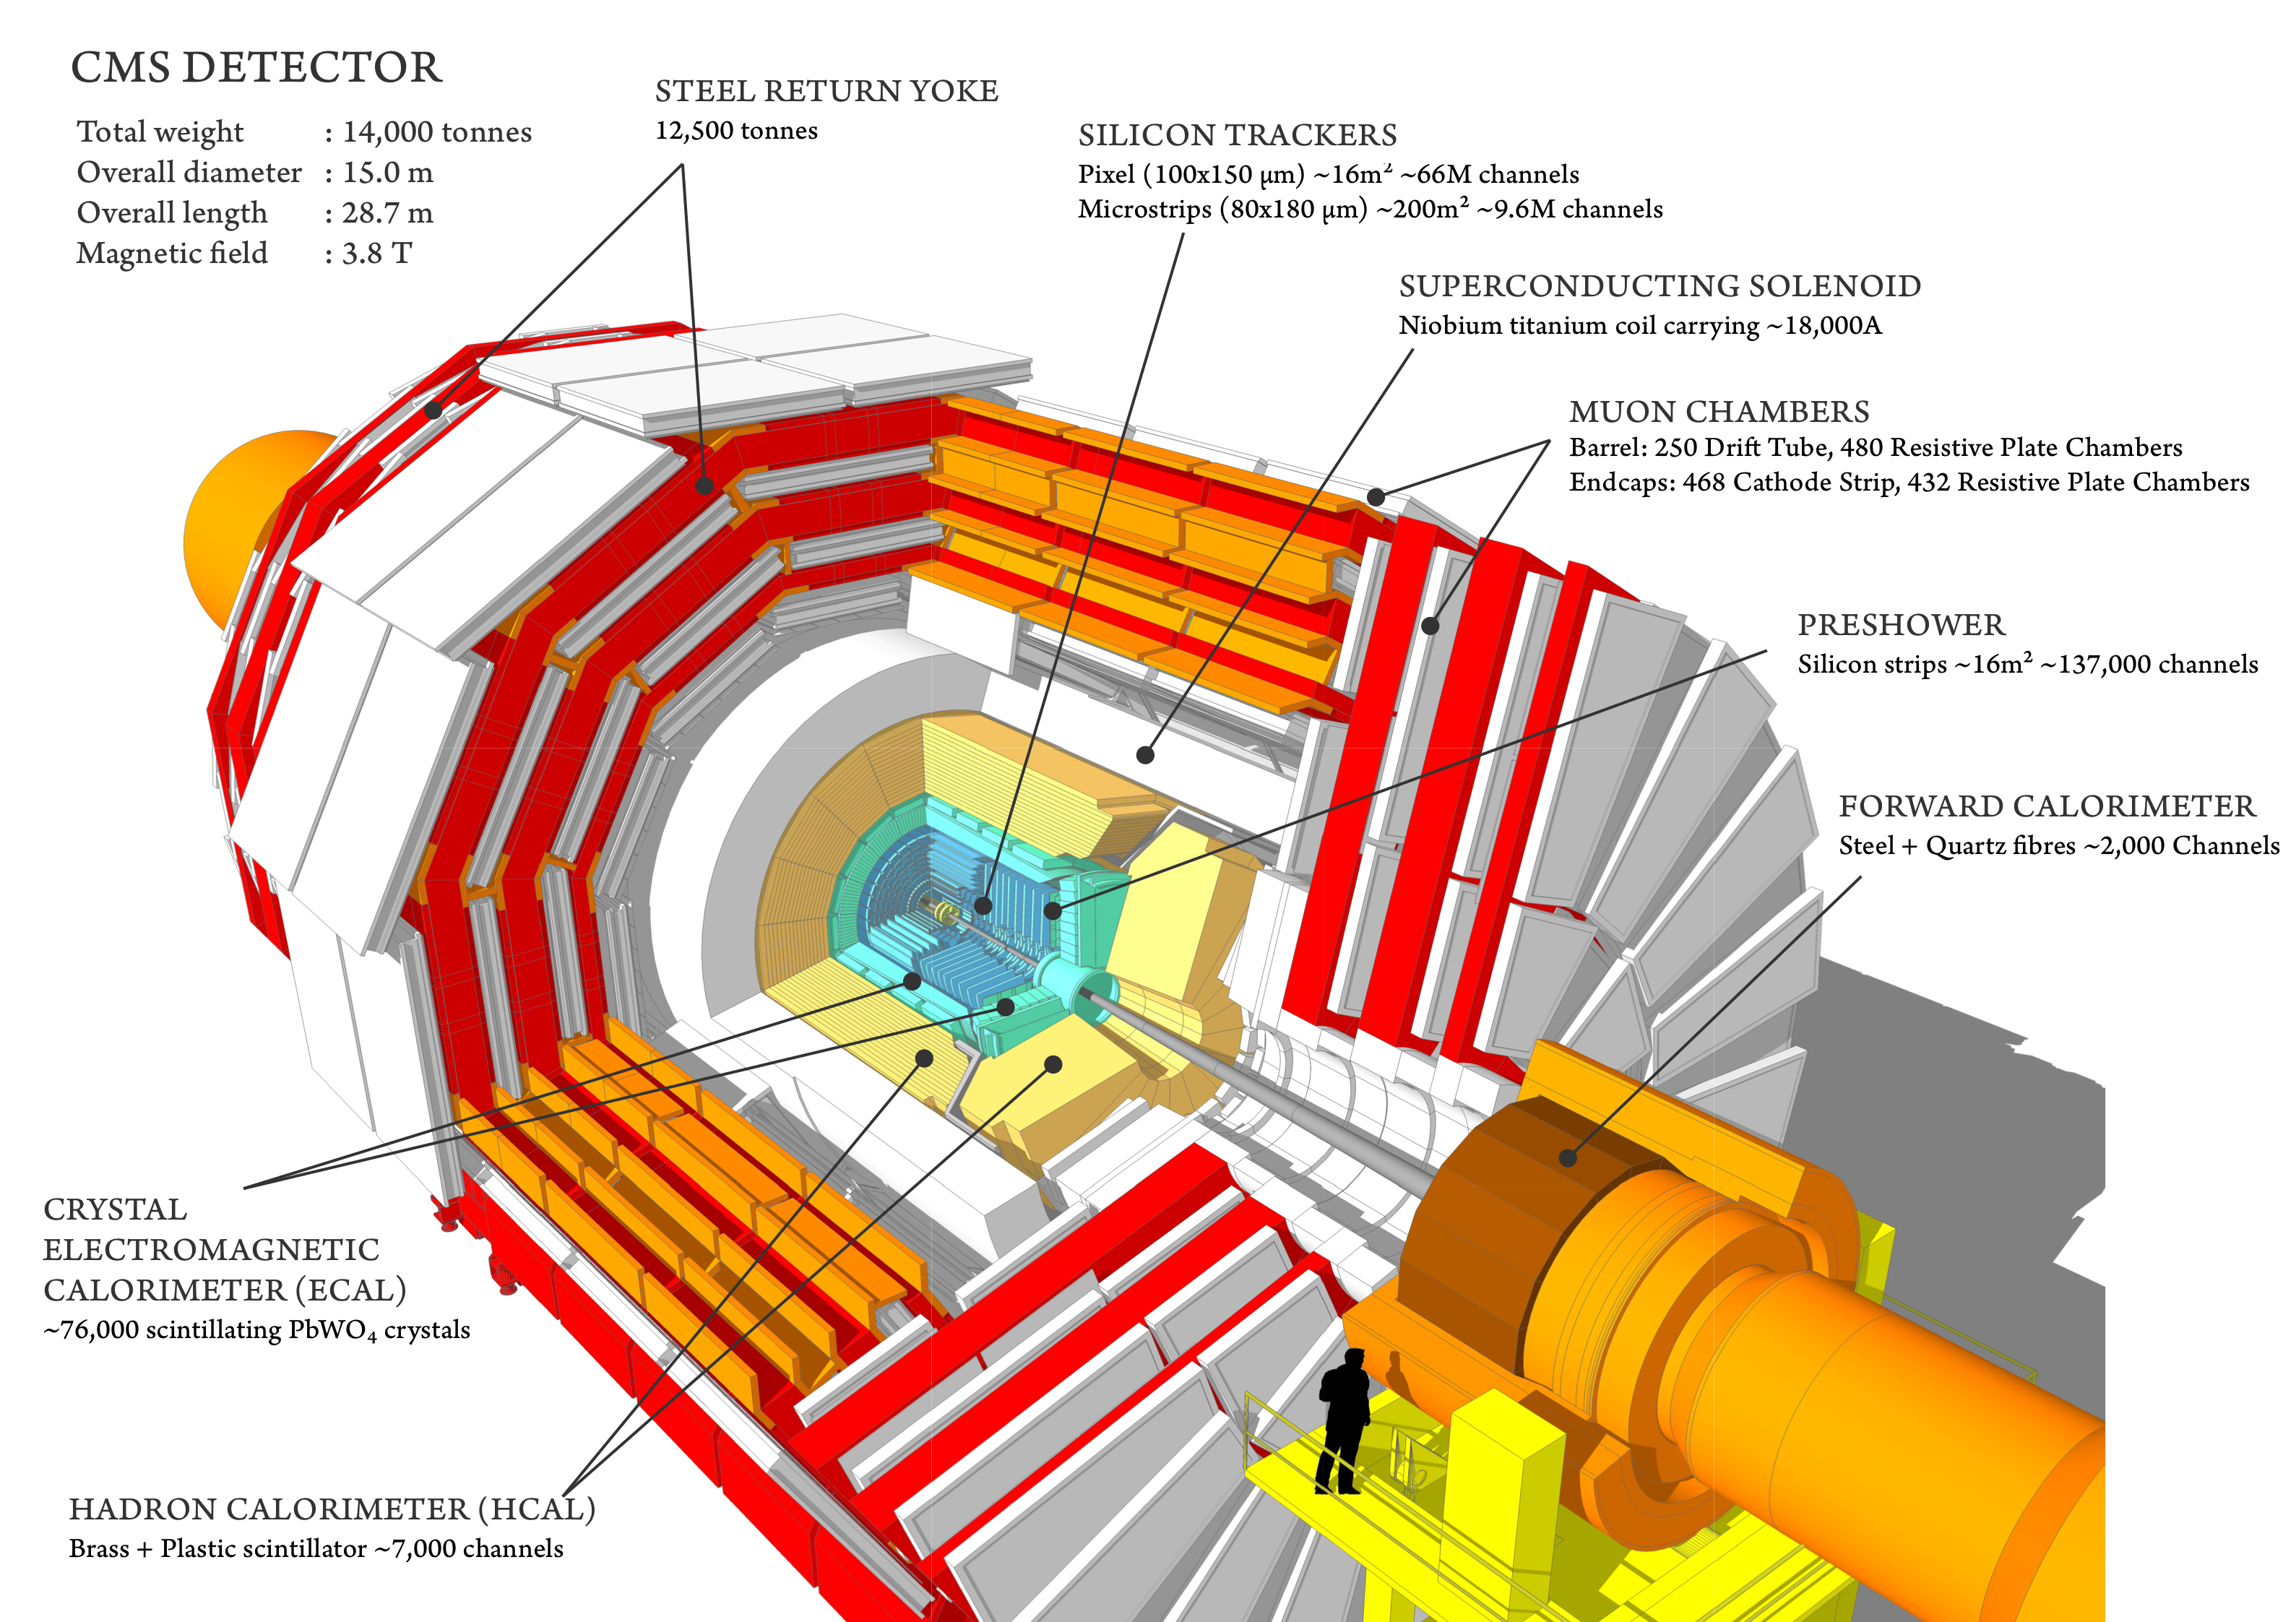
\includegraphics[width=\textwidth]{\figpath/cms.png}
        \end{column}
        \begin{column}{0.35\textwidth}
            \begin{figure}
                \centering
                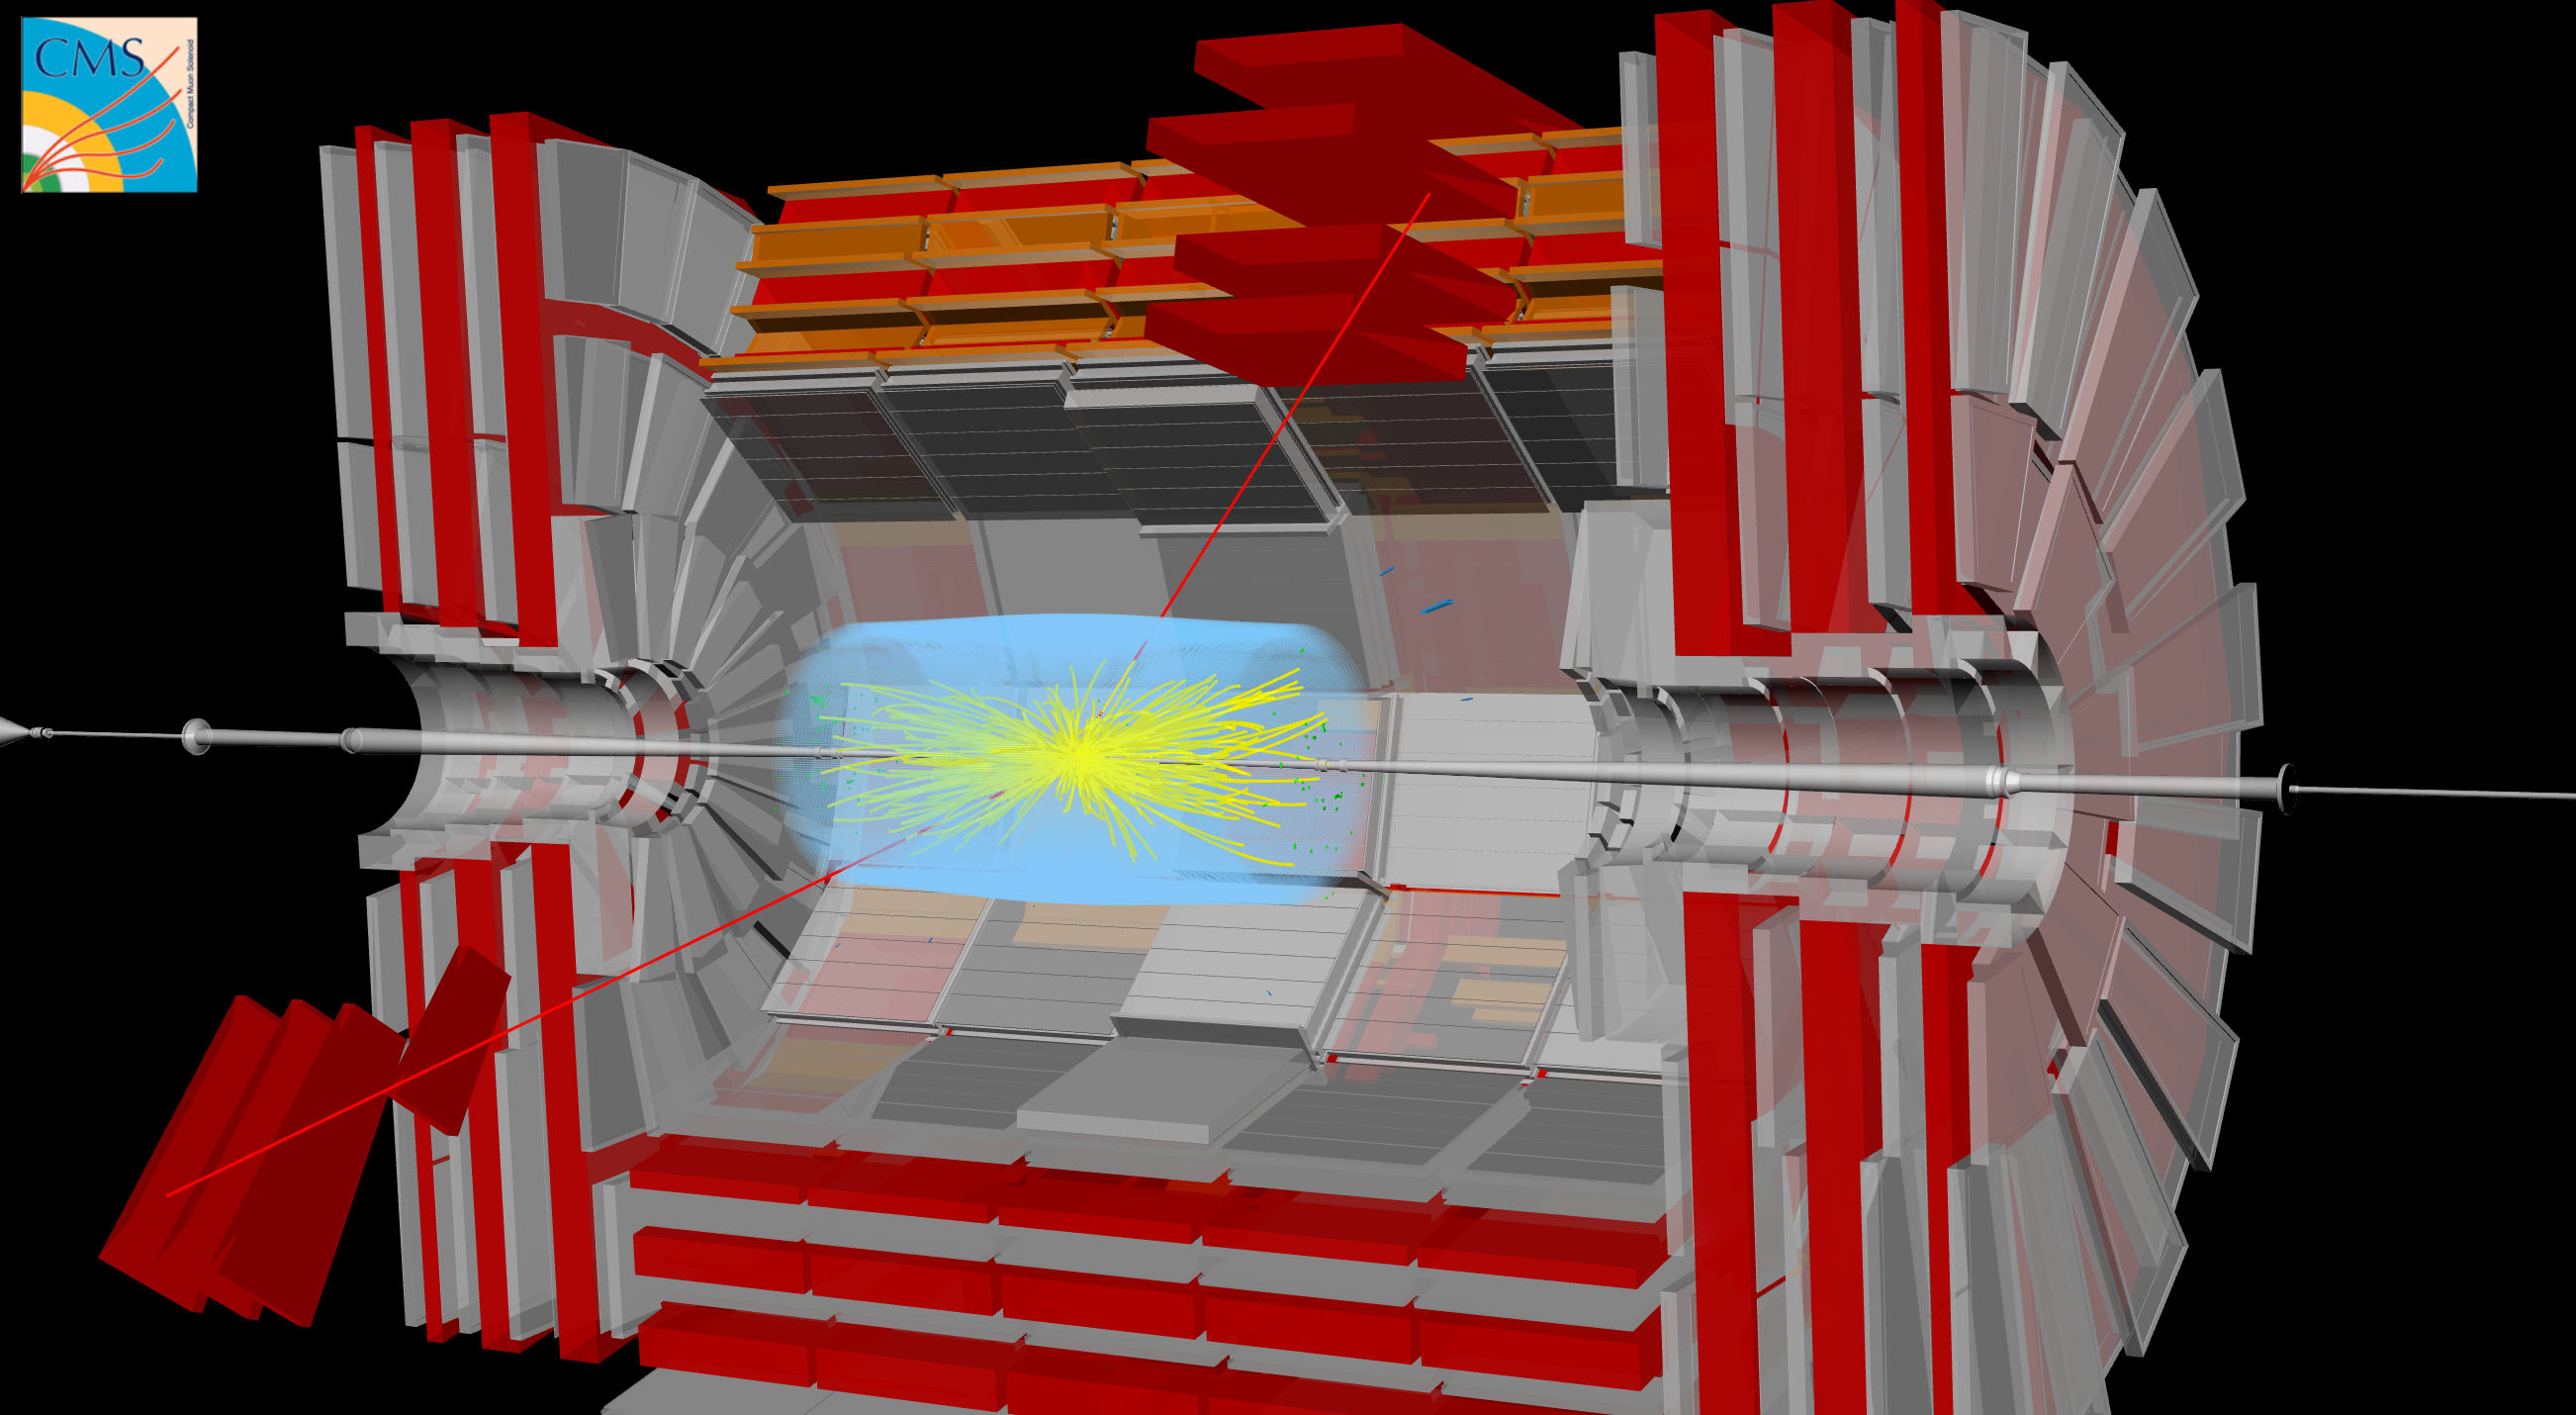
\includegraphics[width=\textwidth]{\figpath/dimuon_logo.png}
            \end{figure}
            \vfill
            \begin{figure}
                \centering
                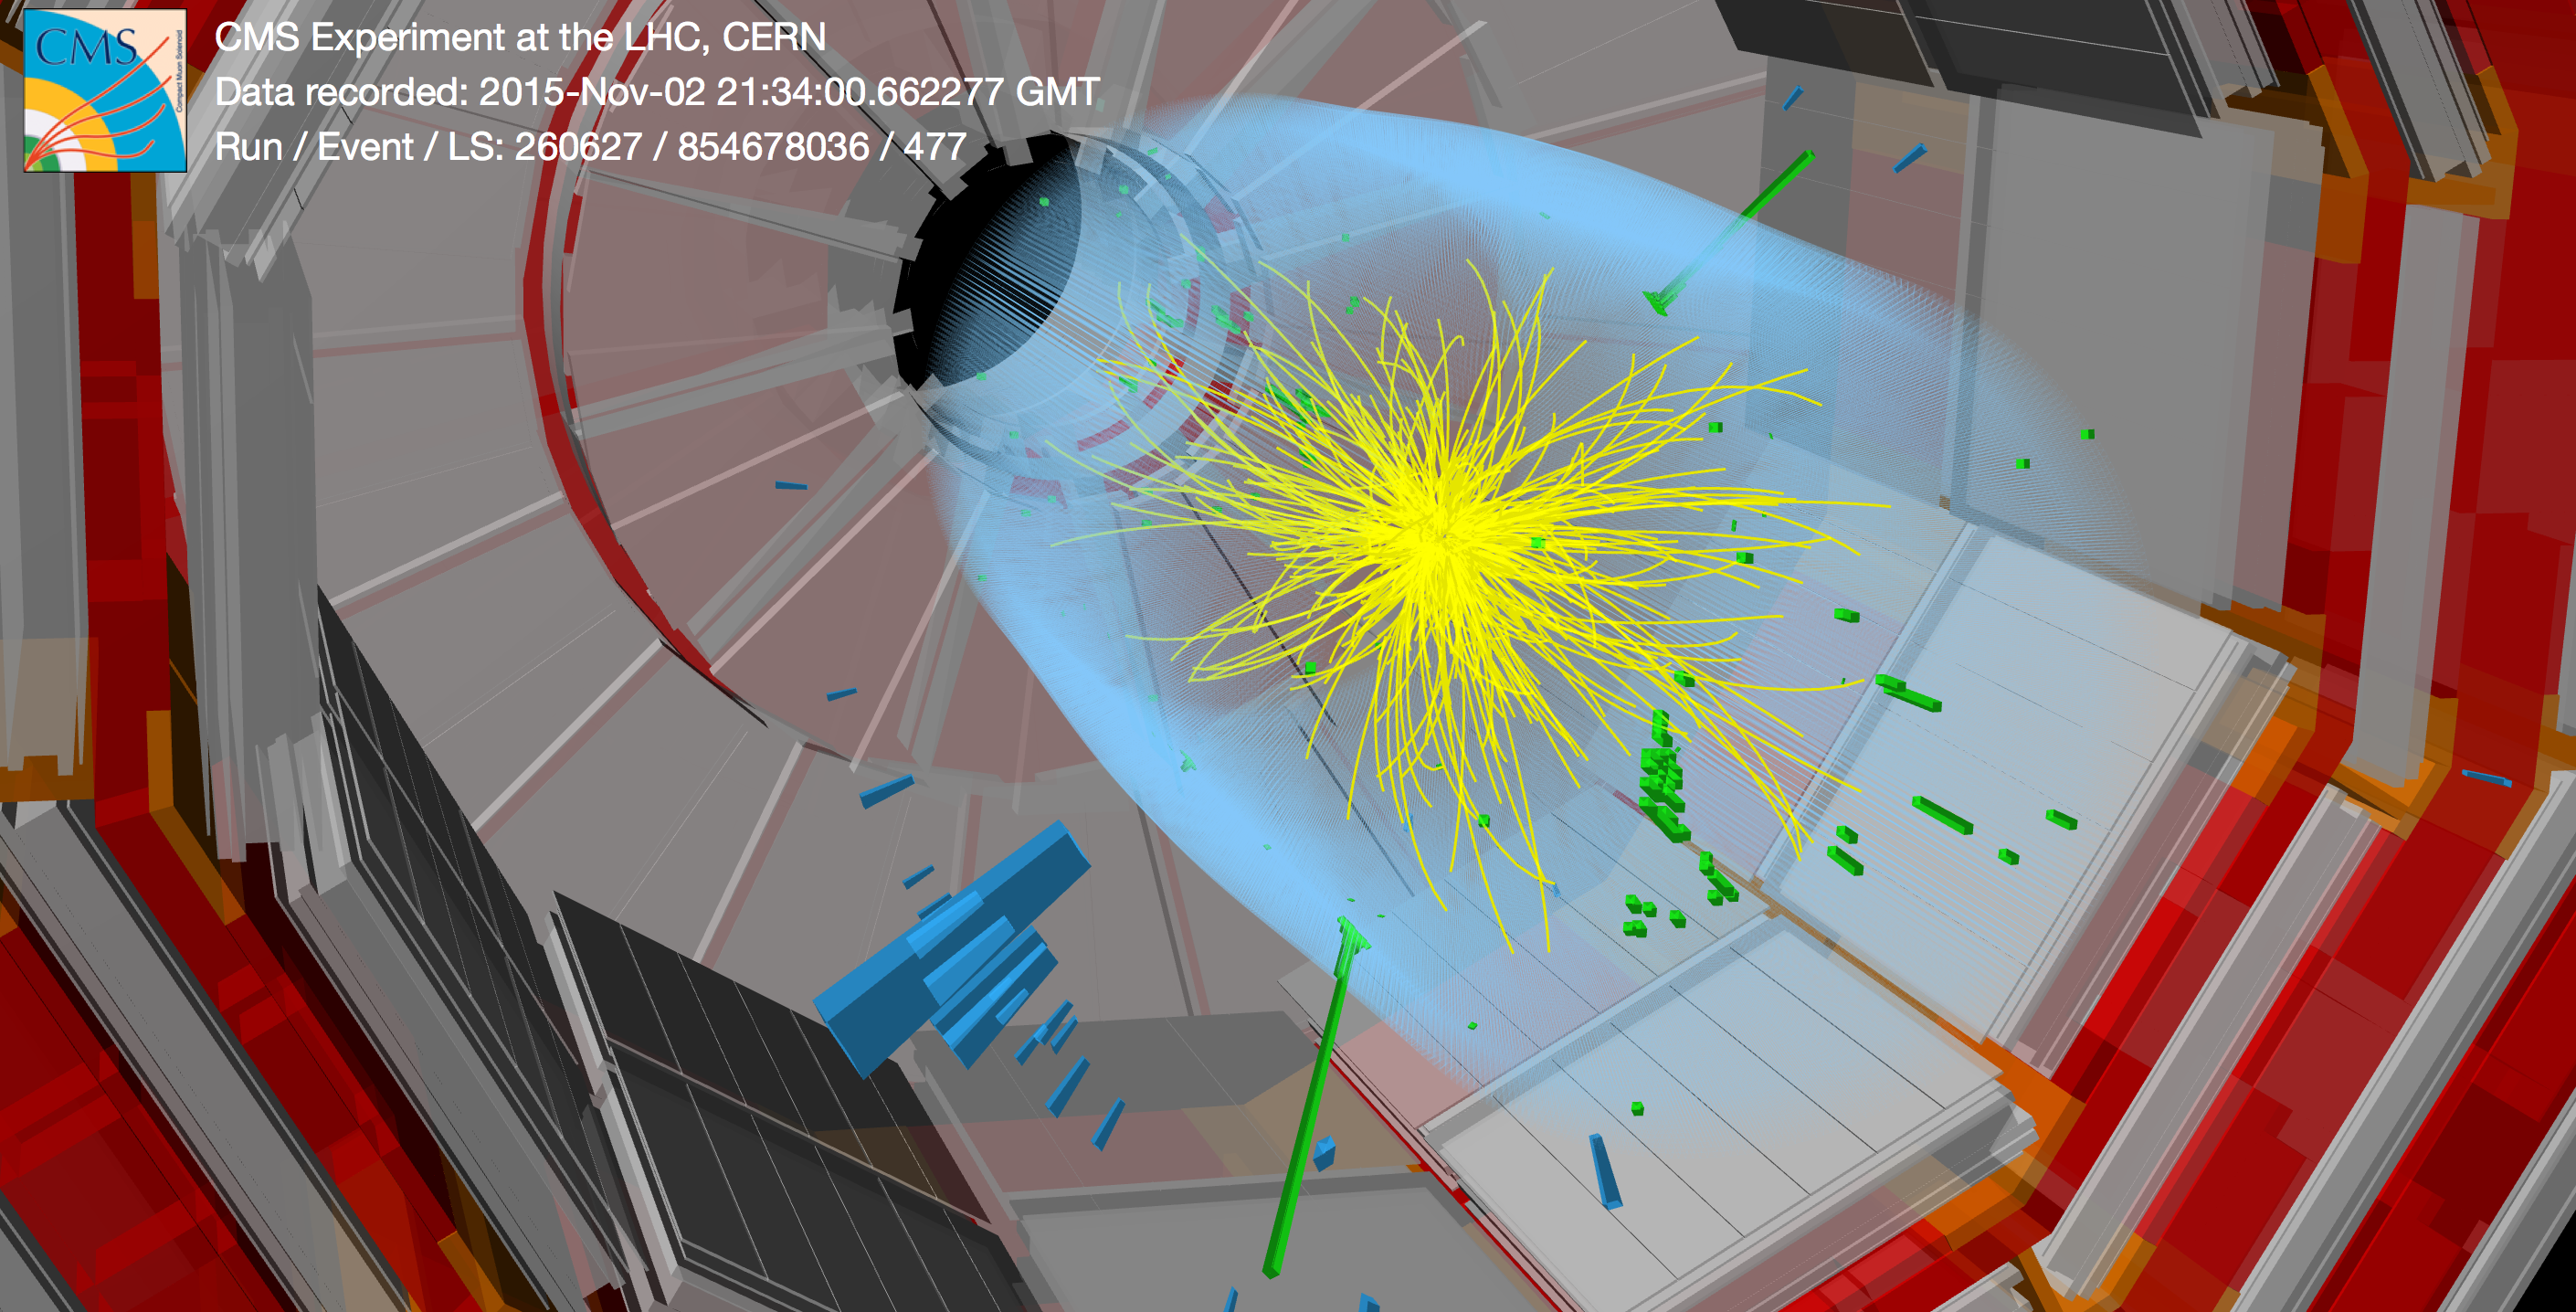
\includegraphics[width=\textwidth]{\figpath/diphoton_v2.png}
            \end{figure}
        \end{column}
    \end{columns}
}

\begin{frame}<1>[label=frame:definitions]
    \setbeamercovered{transparent}
    \frametitle{Definitions}
    \vspace*{-0.24cm}
    \begin{block}{Coordinate System}
        \begin{columns}[T]
            \column{0.5\textwidth}
                \begin{itemize}
                    \scriptsize{
                      \item z-axis - Along the beam pipe
                      \item $\phi$ - The azimuthal angle
                      \item $\eta=-ln[tan(\frac{\theta}{2})]$
                      \item $p_{T}$ - The transverse momentum (in the x-y plane)
                    }
                \end{itemize}
            \column{0.5\textwidth}
                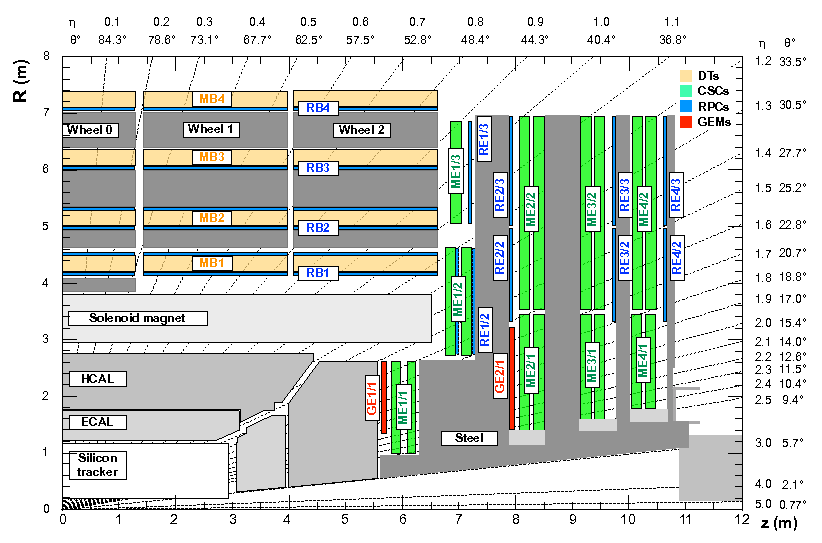
\includegraphics[width=0.53\textwidth]{\figpath/gem_sketch.png}
                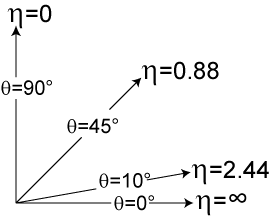
\includegraphics[width=0.45\textwidth]{\figpath/Pseudorapidity2.png}
        \end{columns}
    \end{block}
    \vspace*{-0.16cm}
    \begin{block}{Physics Objects}
        \begin{columns}[T]
            \column{0.45\textwidth}
                \begin{itemize}
                    \scriptsize{
                        \uncover<2->{\item Leptons {\color{gray}(Hadrons/Photons)}}
                        \uncover<3->{\item $\Em_{T}$ - Missing transverse energy
                        \begin{itemize}
                            \scriptsize{
                                \item Intrinsically from neutrinos
                                \item Indirectly from:
                                \begin{itemize}
                                    \scriptsize
                                    \item Jet Mismeasurements
                                    \item Detector Noise
                                    \item Pileup (multiple hard scatter interactions per bunch crossing)
                                \end{itemize}
                            }
                        \end{itemize}}
                        \uncover<4->{\item Jet - Collimated spray of particles
                        \begin{itemize}
                            \scriptsize{
                                \item Resulting from the hadronization of quarks and gluons
                            }
                        \end{itemize}}
                    }
                \end{itemize}
            \column{0.55\textwidth}
                \vspace*{-0.15cm}
                \begin{center}
                    \only<1-2>{\vspace*{0.25cm}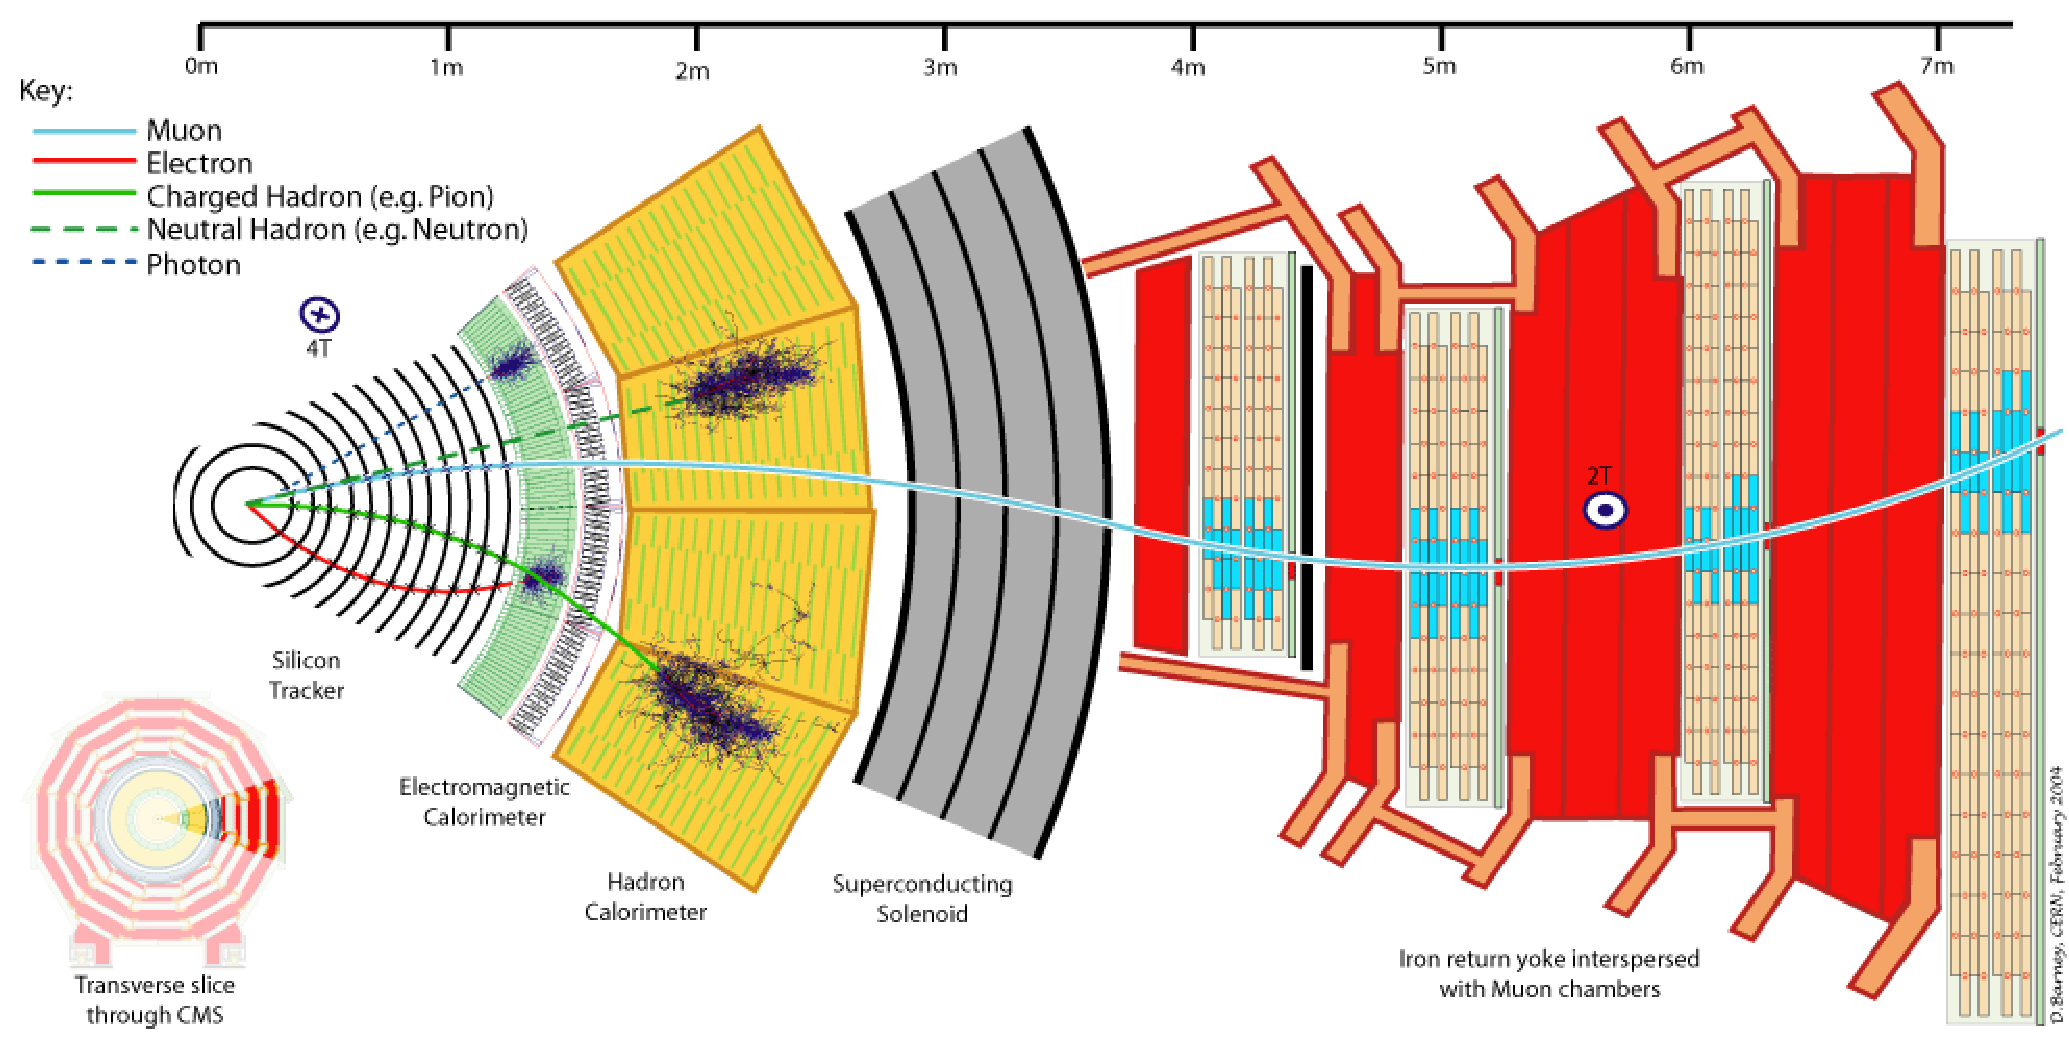
\includegraphics[width=\textwidth]{\figpath/CMS_Slice.pdf}}
                    \only<3>{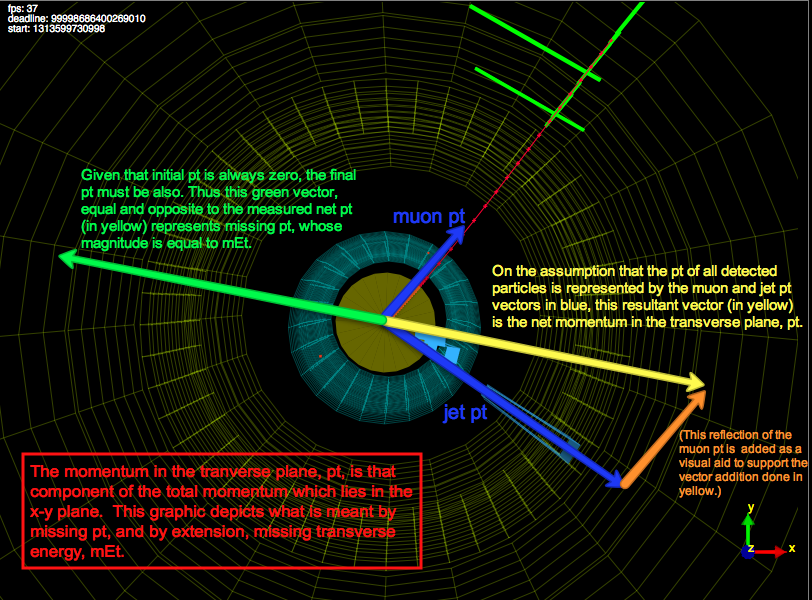
\includegraphics[width=0.8\textwidth]{\figpath/MEt.png}}
                    \only<4>{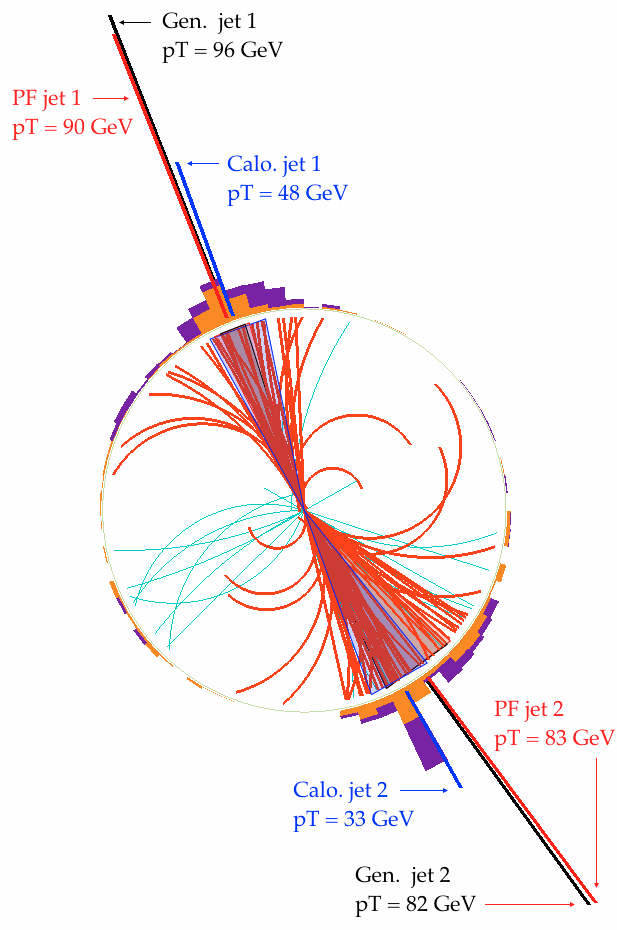
\includegraphics[width=0.4\textwidth]{\figpath/display_xy_annotated.png}}
                    %\only<5>{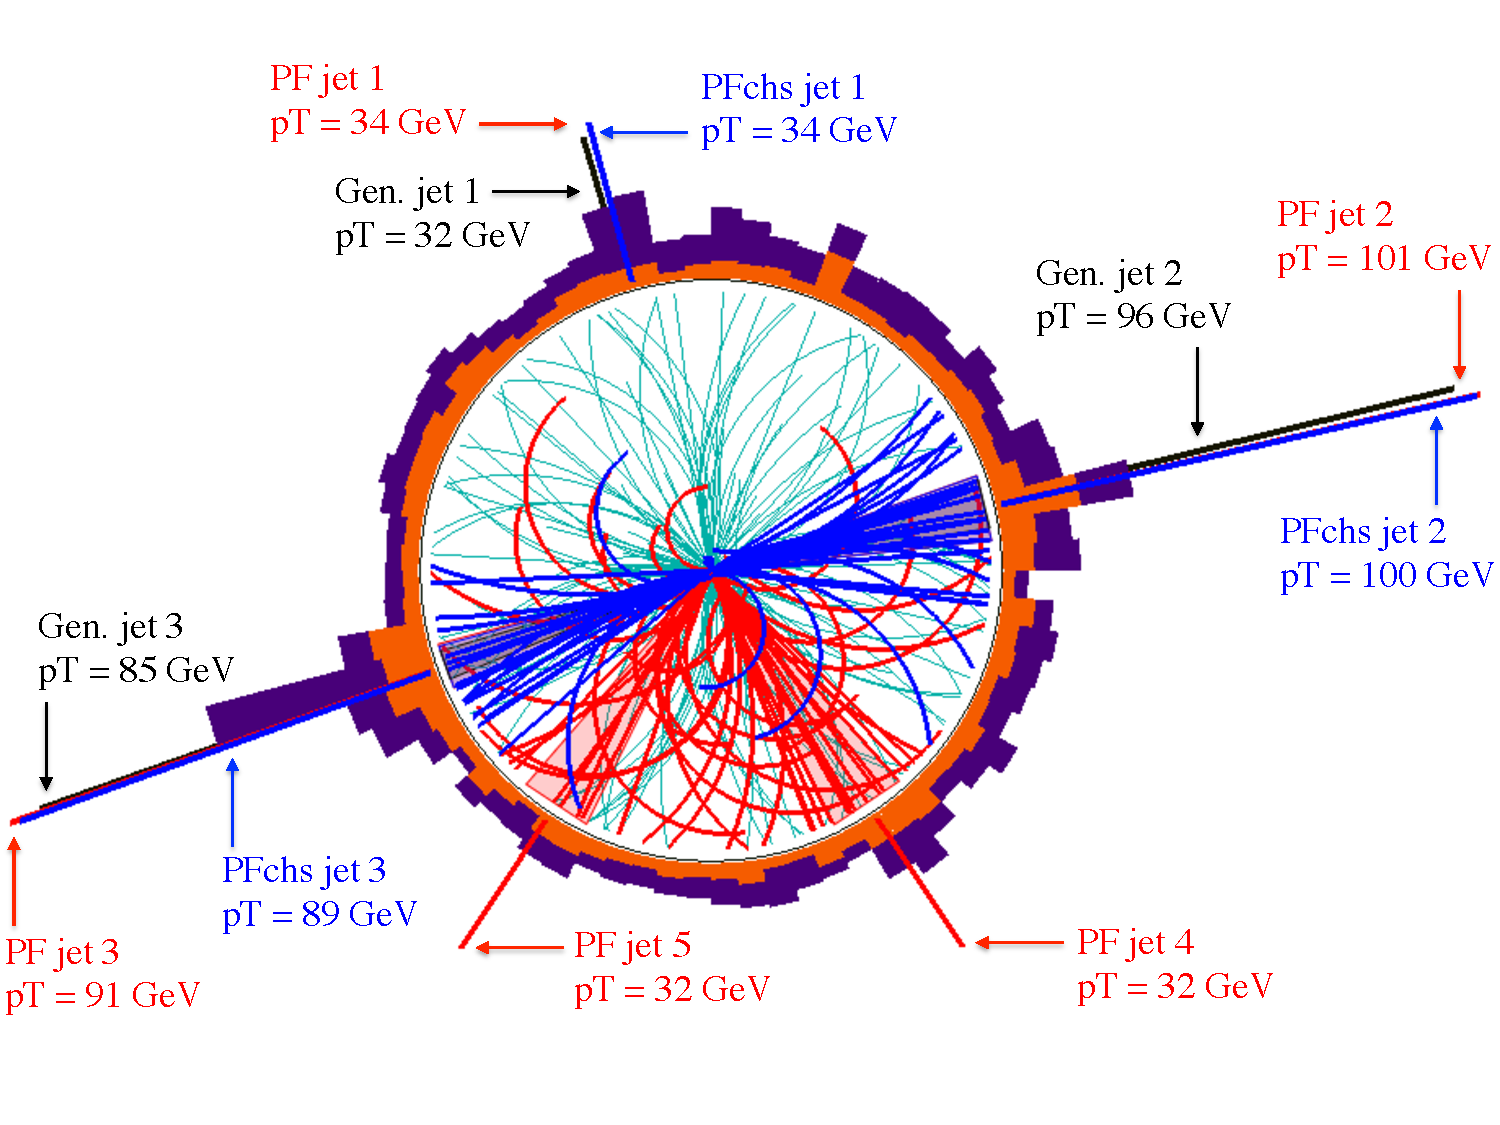
\includegraphics[width=0.8\textwidth]{\figpath/EventDisplay_Run1_Lumi12454_Event1822481_RhoPhi_PFParticles_annotated.pdf}}
                \end{center}
        \end{columns}
    \end{block}
\end{frame}

\againframe<2>{frame:definitions}
\againframe<3>{frame:definitions}
\againframe<4>{frame:definitions}
%\againframe<5>{frame:definitions}